

分布式系统不仅可以运行的孤立实例,也相互沟通,两种方式可以进行适当地整合。

关于集成的主题已经讨论了很多,因此在本节中,将尝试展示一些模式,用于集成全新的系统,以及如何使系统的新组件与现有组件(通常是遗留部分)共存。

为了不使本章的体量成为一本书,这里会对现有的相关书籍进行推荐。如果对集成模式感兴趣,特别是消息传递,那么Gregor Hohpe和Bobby Woolf的《企业集成模式》是必读的。

来简要地看一下本书介绍的两个模式。

\subsubsubsection{4.4.1\hspace{0.2cm}管道与过滤器模式}

第一个集成模式叫做\textbf{管道与过滤器},其目的是将一个大的处理任务分解为一系列较小的、独立的任务(称为过滤器),然后可以将这些任务连接在一起(使用管道,如消息队列)。这种方法有较好的可扩展性、性能和可重用性。

假设需要接收和处理传入的订单。当然,可以在一个大模块中完成,所以不需要额外的通信,但这样一个模块很难测试其不同的功能,也很难对其进行扩展。

不过,可以将订单处理分成多个单独的步骤,每个步骤由一个不同的组件处理:一个用于解码,一个用于验证,另一个用于实际处理订单,然后还有一个用于存储订单。使用这种模式,就可以单独执行这些步骤中的每一个,在需要时可以轻松地替换或禁用,并重用它们来处理不同类型的输入消息。

如果希望同时处理多个订单,还可以流水线处理:一个线程验证消息,另一个线程解码下一个消息,以此类推。

缺点是需要使用同步队列作为管道,这会带来一些开销。

要扩展处理的步骤,可能需要将此模式与管道中的下一个步骤一起使用。

\subsubsubsection{4.4.2\hspace{0.2cm}使用者竞争}

使用者竞争的思想很简单:有一个输入队列(或消息传递通道)和几个从队列中,并发获取和处理项的使用者实例。每个使用者都可以处理消息,因此他们相互竞争成为接收者。

通过这种方式,可以获得可扩展性、自由负载平衡和弹性。添加了队列之后,现在还拥有了基于队列的负载均衡模式。

如果要减少请求的延迟,或者只是希望以更紧急的方式执行提交到队列的特定任务,则此模式可以轻松地与优先级队列集成。

\begin{tcolorbox}[colback=blue!5!white,colframe=blue!75!black, title=Note]
\hspace*{0.7cm}如果顺序很重要,那么使用这种模式可能会很棘手。用户接收和完成消息处理的顺序可能不同,因此要确保这不会影响您的系统,或者可以找到一种方法在以后重新排列结果。如果需要按顺序处理消息,则可能无法使用此模式。
\end{tcolorbox}

现在,为了帮助集成现有的系统,来继续了解更多的模式。

\subsubsubsection{4.4.3\hspace{0.2cm}从遗留系统的过渡}

从头开始开发一个系统是幸福的。开发不是维护,有了使用前沿技术的可能性——为什么不喜欢的呢?不幸的是,当与现有的遗留系统开始集成时,这种幸福就结束了。幸运的是,有一些方法可以缓解这种痛苦。

\hspace*{\fill} \\ %插入空行
\noindent
\textbf{防腐层}

引入\textbf{防腐层}可以让解决方案与具有不同语义的遗留系统,进行无痛的集成。这层负责双方之间的通信。

这样的组件可以让解决方案有更大的灵活性——而不需要损害技术堆栈或架构决策。要实现这一点,只需要在遗留系统中进行最小的更改(如果遗留系统不需要调用新系统,则不需要进行更改)。

例如,如果解决方案是基于微服务的,那么遗留系统可以只与防腐层通信,而不是直接定位和到达每个微服务。转换(例如,由于过时的协议版本)也在这层中完成。

请记住,添加这样的层可能会引入延迟,并且必须满足解决方案的质量属性,例如可扩展性。

\hspace*{\fill} \\ %插入空行
\noindent
\textbf{扼杀者模式}

\textbf{扼杀器模式}允许从遗留系统逐步迁移到新系统。刚才看到的防腐层对于两个系统之间的通信很有用,而扼杀者模式则用于从两个系统向外部提供服务。

迁移过程的早期,扼杀器将把大多数请求放到遗留系统中。在迁移过程中,越来越多的调用可以转发到新的调用中,同时越来越多地限制遗留系统,限制它所提供的功能。作为迁移的最后一步,扼杀器逼迫遗留系统退役——新系统将提供所有的功能:

\begin{center}
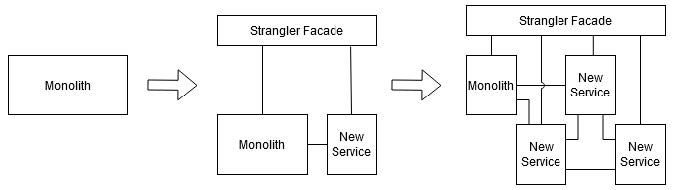
\includegraphics[width=0.9\textwidth]{content/2/chapter4/images/1.jpg}\\
图4.1 - 扼杀者模式。迁移之后,扼杀器仍然可以用作遗留请求的入口点或适配器
\end{center}

对于小型系统,这种模式可能有些大材小用。如果数据存储是共享的,或者是用于事件源系统,这时这种模式会变得棘手。在将其添加到解决方案时,请提前为实现适当的性能和可扩展性做好计划。

接下来,了解一些有助于实现这两个属性的方式。















